\documentclass[times, utf8, seminar, numeric]{fer}
\usepackage{array}
\newcolumntype{P}[1]{>{\centering\arraybackslash}p{#1}}
\usepackage{booktabs}
 \usepackage{url}
\usepackage{indentfirst}

\newcommand\floor[1]{\lfloor#1\rfloor}
\newcommand\ceil[1]{\lceil#1\rceil}

\begin{document}

% Ukljuci literaturu u seminar
\nocite{*}

% TODO: Navedite naslov rada.
\title{Računanje najduljeg zajedničkog prefiksa temeljeno na BWT}

% TODO: Navedite vaše ime i prezime.
\author{Silvestar Badak, Tomislav Gudelj, Domagoj Vukadin}

% TODO: Navedite ime i prezime voditelja.
\voditelj{doc. dr. sc. Mirjana Domazet-Lošo}

\maketitle

\tableofcontents

\chapter{Uvod}
Bioinformatika je grana računarstva koja proučava specifične algoritme i strukture podataka kako bi ih mogli primijeniti u području biologije živih bića. Gen je osnovna jedinica nasljeđivanja u živim organizmima. Sastavni je dio DNA i sastoji se od niza nukleotida (\textit{dušična baza - A,C,G,T, šećera i fosfatne skupine}). Kodirana mRNA dobivena iz gena procesom transkripcije služi za sintezu proteina (\textit{procesom translacije}) koji se sastoje od niza aminokiselina. Proteini obavljaju mnogobrojne funkcije unutar živih bića (\textit{npr. ubrzavaju metaboličke reakcije, služe za transport molekula, umnažanje i prepisivanje DNA, itd.}). Jedan od najpoznatijih proteina je hemoglobin koji je odgovoran za prijenos atoma kisika u krv.\cite{domazet_sikic_skripta} \\
\par Prilikom procesa razmnožavanja živih bića, jedna mala mutacija, tj. promjena jednog nukleotida može rezultirati ozbiljnim posljedicama i obilježiti cijeli životni vijek nastalog organizma. Neke se bolesti uzrokovane mutacijom gena i naslijeđenim genima mogu predvidjeti iz ljudske DNA, koja je jedinstveni identifikator svakog organizma. Sekvenciranjem genoma, skupa svih gena nekog organizma, dobivamo sveukupnu nasljednu informaciju organizma. Genomi su izrazito veliki i nemoguće ih je analizirati bez korištenja računalnih programa, tj. strojeva za analizu. Algoritmi i strukture podataka koji su proizašli iz bioinformatičke znanosti sastavni su dijelovi tih programa i omogućavaju nam da u razumnom vremenu dobijemo informaciju koju želimo. Jedan od takvih programa koji se koristi u analizi genoma je \textbf{računanje najduljeg zajedničkog prefiksa temeljeno na Burrows-Wheelerovoj transformaciji} što je tema ovog projekta. U nastavku slijedi opis korištenih algoritama i struktura podataka.

\chapter{Strukture podataka i algoritmi}
Računanje najduljeg zajedničkog prefiksa izračunatih sufiksa ulaznog niza - $LCP$ u razumnom vremenu može se obaviti na sljedeći način:

\begin{center}
	\begin{enumerate}
		\setlength\itemsep{-0.8em}
		\item {određivanjem \textbf{sufiksnog polja} $SA$ ulaznog niza $S$}
		\item {računanjem \textbf{Burrows-Wheelerove transformacije - BWT} koristeći $SA$}
		\item {izgradnjom \textbf{binarnog stabla valića} nad novim nizom $S'= BWT(S)$}
		\item {implementacijom funkcije \textbf{rang} nad binarnim stablom valića koja se koristi u \textbf{algoritmu 1}}
		\item {konstrukcijom \textbf{LCP polja} \textbf{algoritmom 2} koji poziva metodu $getIntervals$ \textbf{algoritma 1}}
	\end{enumerate} 
\end{center}


\section {Sufiksno polje}
Sufiksno polje je polje indeksa leksikografski poredanih sufiksa nekog niza $S$. Na primjer, neka je zadan ulazni niz $S = "el\_anele\_lepanelen"$ koji je kao primjer naveden u \cite{Beller2011}. Abeceda ovog niza je leksikografski poredan skup znakova sadržan u $S$ - $\sum = \{\$, \_, a, e, l, n, p\}$. Na kraj niza dodajemo jedinstveni znak $\$$. Leksikografski poredani sufiksi navedenog niza su:


\begin{center}
	\begin{enumerate}
		\setlength\itemsep{-0.8em}
		\item \textbf{$\$$}
		\item \textbf{$\_anele\_lepanelen\$$}
		\item \textbf{$\_lepanelen\$$}
		\item \textbf{$anele\_lepanelen\$$}
		\item \textbf{$anelen\$$}
		\item \textbf{$e\_lepanelen\$$}
		\item \textbf{$el\_anele\_lepanelen\$$}
		\item \textbf{$ele\_lepanelen\$$}
		\item \textbf{$elen\$$}
		\item \textbf{$en\$$}
		\item \textbf{$epanelen\$$}
		\item \textbf{$l\_anele\_lepanelen\$$}
		\item \textbf{$le\_lepanelen\$$}
		\item \textbf{$len\$$}
		\item \textbf{$lepanelen\$$}
		\item \textbf{$n\$$}
		\item \textbf{$nele\_lepanelen\$$}
		\item \textbf{$nelen\$$}
		\item \textbf{$panelen\$$}	
	\end{enumerate} 
\end{center}
Sufiksno polje $SA$ je polje indeksa ulaznog niza kojim započinju gore navedeni sufiksi. Slijedno tome vrijedi 
$SA = [18, 2, 8, 3, 12, 7, 0, 5, 14, 16, 10, 1, 6, 15, 9, 17, 4, 13, 11]$.\cite{Beller2011}

\section {Burrows-Wheelerova transformacija - BWT}
Burrows-Wheelerova transformacija je transformacija ulaznog teksta koja rezultira sažimanjem istoga. Može se odrediti na dva načina definirana u \cite{domazet_sikic_skripta}: 
 
\begin{center}
	\begin{enumerate}
		\setlength\itemsep{-0.8em}
		\item {izravno iz ulaznog niza (rotacijom ulaznog niza $S$)}
		\item {preko sufiksnog polja $SA(S)$}

	\end{enumerate} 
\end{center}

U ovom projektu koristi se drugi način u kojem za ulaz $S = "el\_anele\_lepanelen"$ kao rezultat dobivamo $S' = BWT(S) = "nle\_pl\$nnlleee\_eaae"$ na sljedeći način:

\begin{equation}\label{bwt}
BWT[i] = 
\begin{cases}
S[SA[i] - 1], & \text{ako}\ \forall{i}(SA[i] \neq 0)\\
\$, & \text{inače}
\end{cases}
\end{equation}

\section {Binarno stablo valića}
Binarno stablo valića (\textit{engl. Binary Wavelet Tree}) je struktura podataka novijeg vremena koja nudi rješenja mnogim problemima iz različitih domena kao što su analiza nizova znakova, računalna geometrija i kompresija podataka. Kao ulaz prima niz znakova $S$ koji je sadržan od znakova abecede $\sum$. Omogućava viši stupanj entropije i podržava različite funkcije koje manipuliraju nad ulaznim nizom $S$ značajno brže nego neke klasične funkcije istog izlaza. \cite{wt_book}
\par Stablo valića podržava tri vrste upita: \textbf{pristup} (\textit{engl. access}), \textbf{rang} (\textit{engl. rank}) i \textbf{odabir} (\textit{engl. select}). Funkcija \textit{access(p)} vraća znak \textit{c} koji se nalazi na poziciji \textit{p}, \textit{rank$_p$(c)} broj pojavljivanja znaka \textit{c} do pozicije \textit{p} uključivo, \textit{select$_c$(o)} poziciju znaka \textit{c} nakon \textit{o} pojavljivanja. U ovom se projektu koristi samo funkcija rang o kojoj će biti rečeno nešto više u nastavku.\cite{wt_book} Primjer stabla valića dan je na slici 2.1.
Za konstrukciju čvorova stabla korišten je pseudokod na slici 2.2.

\par Svaki čvor sadrži vektor bitova koji predstavlja trenutni niz dobiven iz prethodnog čvora i definiran je abecedom $\sum^{[l..r]}$, gdje $l$ i $r$ predstavljaju indekse početka i završetka podabecede u početnoj abecedi $\sum^{[0..\sigma]}$ koja pripada korijenu stabla i gdje je $\sigma$ indeks zadnjeg znaka u nizu. Nekom znaku dodjeljujemo vrijednost 0 ako se nalazi u intervalu $[l..m]$ unutar podabecede trenutnog čvora koja sadrži znakove zastupljene samo u tom čvoru, gdje je $m = \frac{\floor{l + r}}{2}$, inače 1 ako se pak nalazi u intervalu $[m + 1..r]$. Čvorovi se granaju u dva smjera: lijevo - svi znakovi koji su dobili vrijednost 0 i desno - svi znakovi koji su dobili vrijednost 1, zajedno sa svojim podabecedama. Grananje prestaje kad se u čvoru nalazi samo jedan bit (niz istih bitova), odnosno kad je vrijednost tog čvora jednoznačna (samo jedan znak). Taj se čvor naziva list. Listova je onoliko koliko abeceda sadrži znakova.\cite{Beller2011}
\begin{center}
	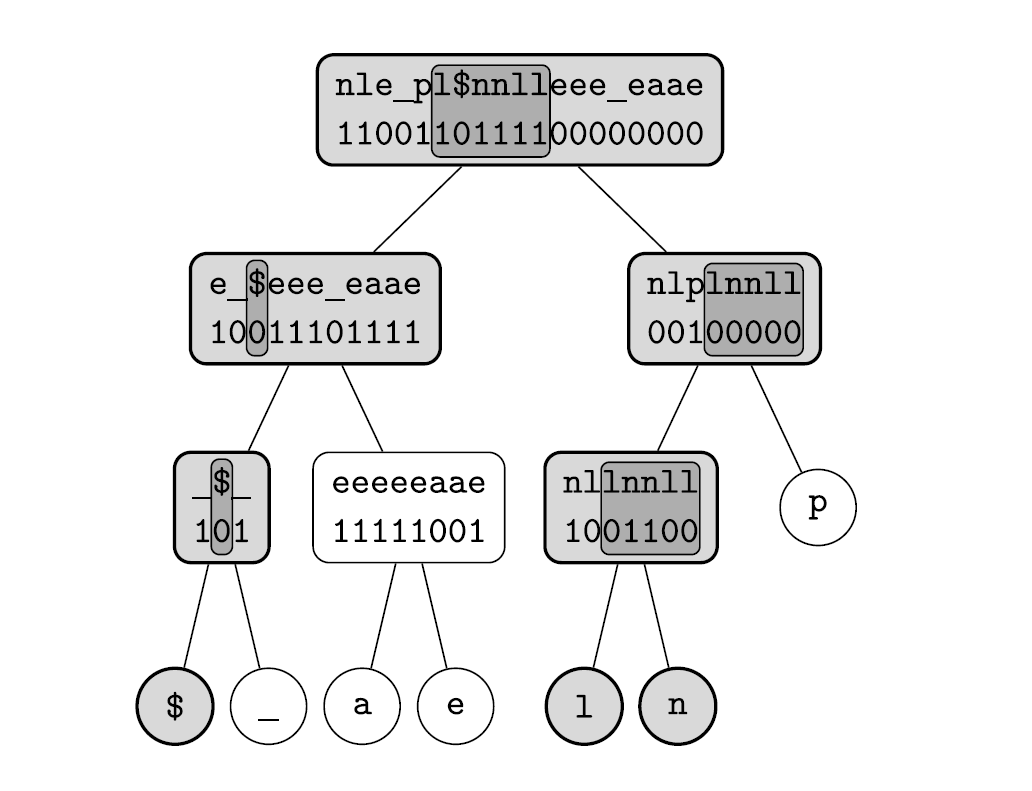
\includegraphics[scale=0.48]{slike/wavelet_tree.png}
	\captionof{figure}{Binarno stablo valića nad nizom $S' = BWT(S) = "nle\_pl\$nnlleee\_eaae"$. Slika preuzeta iz \cite{Beller2011}.}
\end{center}
\begin{center}
	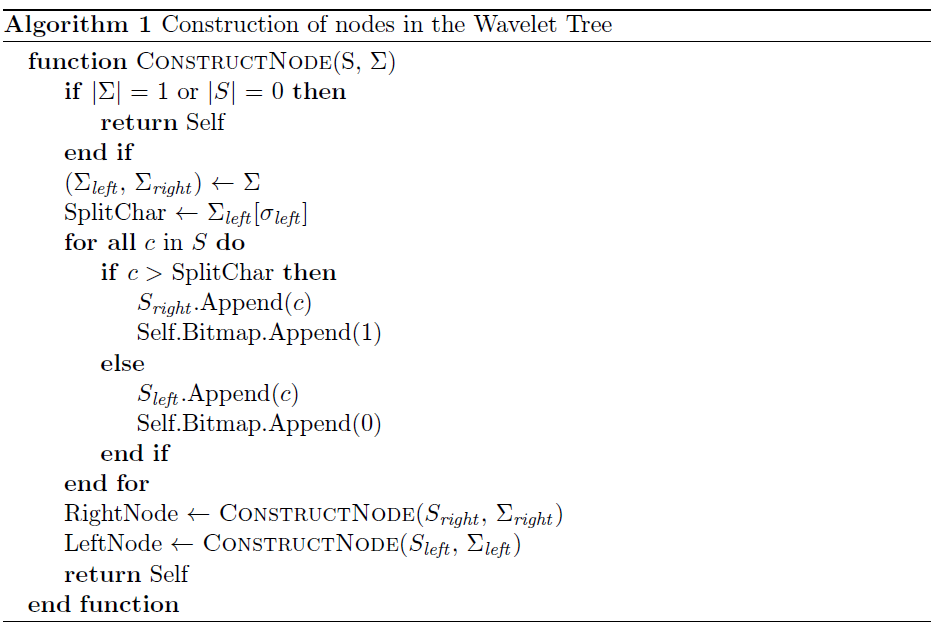
\includegraphics[scale=0.5]{slike/izradnja_wt.png}
	\captionof{figure}{Pseudokod za izgradnju stabla valića. Slika preuzeta iz \cite{wt_book}.}
\end{center}

\par Funkcija rang implementirana je koristeći pseudokod na slici 2.3. Rekurzivna je i efikasno računa broj pojavljivanja znaka do nekog indeksa. Uzmemo li za primjer ulazni niz $S' = BWT(S) = "nle\_pl\$nnlleee\_eaae"$ te nakon konstrukcije stabla pozovemo \textit{rank$_p$(c)}, vrijednost ćemo dobiti na sljedeći način:

\begin{center}
	\begin{enumerate}
		\setlength\itemsep{-0.8em}
		\item {provjeravamo kojoj skupini (0 ili 1) pripada dani znak}
		\item {funkcijom BinaryRank računamo broj pojavljivanja dobivene skupine iz 1. do danog indeksa u trenutnom čvoru, odnosno indeks koji tražimo za dijete u koje prelazimo}
		\item {ovisno koju smo skupinu dobili u 1. prelazimo u lijevo, odnosno desno dijete}
		\item {ponavljamo od 1. do 3. sve dok 5. nije zadovoljeno}
		\item {kada dođemo do čvora u kojem postoji samo jedan znak rezultat je novoizračunati indeks u prethodnom čvoru plus jedan - povratak iz rekurzija}
		
	\end{enumerate} 
\end{center}


\begin{center}
	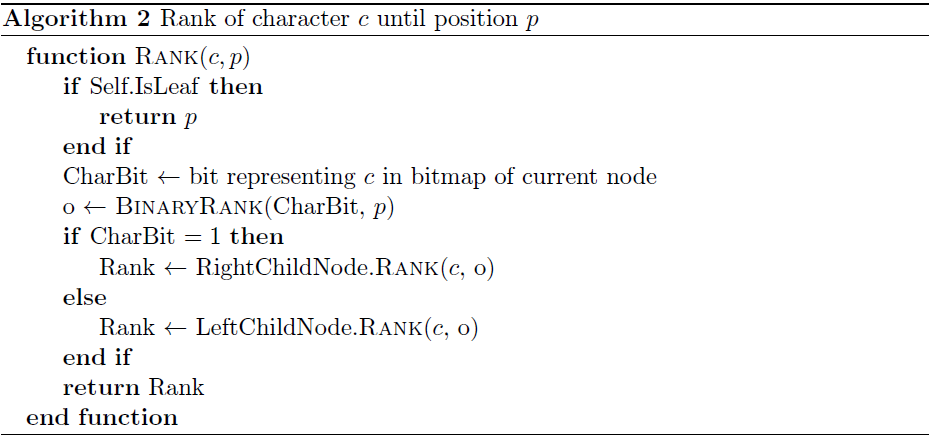
\includegraphics[scale=0.5]{slike/rank.png}
	\captionof{figure}{Pseudokod funkcije rang. Slika preuzeta iz \cite{wt_book}.}
\end{center}

Na primjer \textit{rank$_9$('n')}. Prvi ulazak rezultira novim indeksom 6 i prelazimo u desno dijete (jer 'n' pripada skupini 1 u prvoj podabecedi). Drugi ulazak rezultira novim indeksom 5 te prelazimo u lijevo dijete. Kod trećeg ulaska novi indeks je 2, prelazimo u desno dijete. Desno dijete je jednoznačno i zadovoljen je uvjet 4. te dobivamo rezultat: $index + 1 = 2 + 1 = 3$.

\section{Algoritmi}

Neke analize nizova zahtijevaju polje najdužih zajedničkih prefiksa (\textit{engl. longest common prefix array - $LCP$}). Polje sadržava duljine najdužih zajedničkih prefiksa između svih parova koji su uzastopno poredani u sufiksnom polju. Primjer izračunatog LCP polja prikazan je na slici \ref{lcp_table}.



\begin{center}
	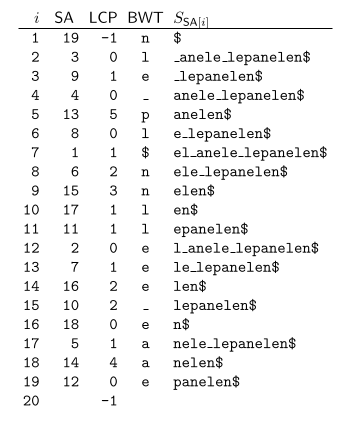
\includegraphics[scale=0.5]{slike/lcp_table.png}
	\captionof{figure}{ Sufiksno polje ($SA$), $BWT$ niz i $LCP$ polje. Slika preuzeta iz \cite{Beller2011}. }
	\label{lcp_table}
\end{center}


U ovom radu obrađuje se implementacija LCP polja temeljena na BWT transformaciji. Prema radu\cite{Beller2011} najlošije vrijeme izvođenja algoritma je $ O(n\hspace{0.5mm} log \hspace{0.5mm} \sigma) $. Algoritmi 1 i 2 za  izračunavanje LCP polja objašnjeni su u nastavku.

\subsection{Algoritam 1}
Feragina  i Manzini u članku\cite{feragina} pokazuju kako je moguće pretraživati uzorke u sufiksnom polju unazad znak po znak bez spremanja sufiksnog polja u memoriju. Neka je $\omega\hspace{0.5mm} \epsilon\hspace{0.5mm} \Sigma $ i $ \omega$ podniz od S. Za $\omega$-interval $[i..j]$ u sufiksnom polju SA niza S ($\omega$ je prefiks svih sufiksa u sufiksnom polju $S_{SA[k]}$ za sve $ i \leq k \leq j $), funkcija \textit{backwardSearch(c, [i..j])} vraća $ c\omega$-interval $[C[c] + Occ(c, i -1) + 1.. C[c] + Occ(c,j) ]$ gdje je $C[c]$ ukupni broj pojavljivanja znakova u S koji su strogo leksikografski manji od $c$, a $Occ(c,i)$ je broj pojavljivanja znaka $c$ u BWT transformaciji u intervalu $[1..i]$.

\subsection{Algoritam 2}

\chapter{Eksperimenti i rezultati}

	  \begin{table}[h]
	  	
	  	\centering
	  	\begin{tabular}{|P{2cm}|P{3cm}|P{2.5cm}|} 
		 \hline
		  Broj znakova & Implementacija Simona Goga [s] & Binarno stablo valića [s] \\
	  		 \hline
	  		100 & 0.037231 & x \\
	  		1,000 & 0.030089 & x \\
	  		10,000 & 0.022991  & x \\ 
	  		100,000 &  0.03929 & x \\
	  		1,000,000 & 0.223351 & x \\	
	  		
	  		\hline  		
	  	\end{tabular}
	  	\caption{Brzine izvođenja}
	  	\label{tbl:std_dev}
	  \end{table}

asd


\chapter{Zaključak}
Zaključak.

\bibliography{literatura}
\bibliographystyle{fer}

\chapter{Sažetak}
Sažetak.

\end{document}
